%-------- Document Class  ------------------------------------------------------------------------------------------------------------------------------------------------
\documentclass[a4paper,11pt]{scrartcl}
\usepackage[margin=1cm
%,showframe% <- only to show the page layout
]{geometry}
\usepackage[utf8]{inputenc}
%-------- Multi-file  ---------------------------------------------------------------------------------------------------------------------------------------------------------
\usepackage{subfiles}

%-------- Preambolo  --------------------------------------------------------------------------------------------------------------------------------------------------
%Per le Figure
\usepackage[english]{babel}
\usepackage{graphicx}

%simboli matematici strani quali unione disgiunta
\usepackage{amssymb}

%Scrivere Sotto i simboli
\usepackage{amsmath}

%Diagrammi Commutativi
\usepackage{tikz}
\usetikzlibrary{matrix}

%Il simbolo di Identità
\usepackage{dsfont}

%Per riflettere i simboli...
\usepackage{graphicx}


%link iNTERNET
\usepackage{hyperref}

%Enumerate with letters
\usepackage{enumerate}

%Slash over letter
\usepackage{cancel}

%Usare bibiliografia bibtex
%\bibliographystyle{plain}

%Danger sign
\usepackage{fourier}

%:=
\usepackage{mathtools}

%http://tex.stackexchange.com/questions/8625/force-figure-placement-in-text
\usepackage{caption}


%subsection numbering
 \setcounter{tocdepth}{3} % if you want all the levels in your table of contents

%Common symbols
%Common math symbols
	%Number fields
		\newcommand{\Real}{\mathbb{R}}
		\newcommand{\Natural}{\mathbb{N}}
		\newcommand{\Relative}{\mathbb{Z}}
		\newcommand{\Rational}{\mathbb{Q}}
		\newcommand{\Complex}{\mathbb{C}}
	
%equality lingo
	%must be equal
		\newcommand{\mbeq}{\overset{!}{=}} 

% function
	%Domain
		\newcommand{\dom}{\mathrm{dom}}
	%Range
		\newcommand{\ran}{\mathrm{ran}}
	

% Set Theory
	% Power set (insieme delle parti
		\newcommand{\PowerSet}{\mathcal{P}}

%Differential Geometry
	% Atlas
		\newcommand{\Atlas}{\mathcal{A}}
	%support
		\newcommand{\supp}{\textrm{supp}}

	
	
%Category Theory
	%Mor set http://ncatlab.org/nlab/show/morphism
%		\newcommand{\hom}{\textrm{hom}}

%Geometric Lagrangian Mechanics
	% Kinematic Configurations
		\newcommand{\Conf}{\mathtt{C}}
	%Solutions Space
		\newcommand{\Sol}{\mathtt{Sol}}
	%Lagrangian class
		\newcommand{\Lag}{\mathsf{Lag}}
	%Lagrangiana
		\newcommand{\Lagrangian}{\mathcal{L}}
	%Data
		\newcommand{\Data}{\mathsf{Data}}
	%unique solution map
		\newcommand{\SolMap}{\mathbf{s}}
	%Classical Observables
		\newcommand{\Obs}{\mathcal{E}}	
	%Phase Space
		\newcommand{\Phase}{\mathcal{M}}	

		\
		
%Peierls (per non sbagliare più)
		\newcommand{\Pei}{Peierls}

%Accented Letters
\usepackage[utf8]{inputenc}

%Temporaneo, Aggiunta della mia classe teorem... Deve diventare un pacchetto!
\input{../Latex-Theorem/TheoremTemplateToninus.tex}
%Common math symbols
	%Number fields
		\newcommand{\Real}{\mathbb{R}}
		\newcommand{\Natural}{\mathbb{N}}
		\newcommand{\Relative}{\mathbb{Z}}
		\newcommand{\Rational}{\mathbb{Q}}
		\newcommand{\Complex}{\mathbb{C}}
	
%equality lingo
	%must be equal
		\newcommand{\mbeq}{\overset{!}{=}} 

% function
	%Domain
		\newcommand{\dom}{\mathrm{dom}}
	%Range
		\newcommand{\ran}{\mathrm{ran}}
	

% Set Theory
	% Power set (insieme delle parti
		\newcommand{\PowerSet}{\mathcal{P}}

%Differential Geometry
	% Atlas
		\newcommand{\Atlas}{\mathcal{A}}
	%support
		\newcommand{\supp}{\textrm{supp}}

	
	
%Category Theory
	%Mor set http://ncatlab.org/nlab/show/morphism
%		\newcommand{\hom}{\textrm{hom}}

%Geometric Lagrangian Mechanics
	% Kinematic Configurations
		\newcommand{\Conf}{\mathtt{C}}
	%Solutions Space
		\newcommand{\Sol}{\mathtt{Sol}}
	%Lagrangian class
		\newcommand{\Lag}{\mathsf{Lag}}
	%Lagrangiana
		\newcommand{\Lagrangian}{\mathcal{L}}
	%Data
		\newcommand{\Data}{\mathsf{Data}}
	%unique solution map
		\newcommand{\SolMap}{\mathbf{s}}
	%Classical Observables
		\newcommand{\Obs}{\mathcal{E}}	
	%Phase Space
		\newcommand{\Phase}{\mathcal{M}}	

		\
		
%Peierls (per non sbagliare più)
		\newcommand{\Pei}{Peierls}    %Common symbols
\usepackage{glossaries}

\makenoidxglossaries

%How to:
%affinchè la voce venga printata nella lista va prima chiamata nel testo come e.g. \gls{Bundle}
%ricordarsi di chiamarlo almeno una volta così, dopo usare il command per evitare il ripetuto hyperref
% anche se si potrebbe evitare visto che il quadratino del link non dovrebbe apparire in stampa

%Advanced Differential Geometry
\newglossaryentry{Bundle}%
{%
	name={\ensuremath{E = (E,\pi , M;Q)}},
	description={ Fiber Bundles $\pi: E\rightarrow M$ with typical fiber $Q$},
    sort={B}
}

\newglossaryentry{Sections}%
{%
	name={\ensuremath{\Gamma^\infty(E)}},
	description={ Smooth sections on the bundle $E$.},
    sort={S}
}


%Geometric Lagrangian Mechanics
	% Kinematic Configurations
	\newglossaryentry{Conf}%
	{%
		name={\ensuremath{\Conf}},
		description={ Kinematic Configurations set}
	}

	%Solutions Space
	\newglossaryentry{Sol}%
	{%
		name={\ensuremath{\Sol}},
		description={ Dynamic Configurations set}
	}

		
	%Lagrangian class
		\newglossaryentry{Lag}%
	{%
		name={\ensuremath{\Lag}},
		description={ Set of Lagrangian densities.}
	}
		
	%Lagrangiana
	\newglossaryentry{Lagrangian}%
	{%
		name={\ensuremath{\Lagrangian}},
		description={ Lagriangian density of the system.}
	}
		
	%Data
	\newglossaryentry{Data}%
	{%
		name={\ensuremath{\Data}},
		description={ Inital Data set.}
	}
		
	%unique solution map
	\newglossaryentry{SolMap}%
	{%
		name={\ensuremath{\SolMap}},
		description={ Map that map a fixed initial data to the unique solution.}
	}
		
	%Classical Observables
	\newglossaryentry{Obs}%
	{%
		name={\ensuremath{\Obs}},
		description={ Set of all classical observables.}
	}

	%Phase Space
	%Classical Observables
	\newglossaryentry{Phase}%
	{%
		name={\ensuremath{\Phase}},
		description={ Phase space.}
	}



\hyphenation{gua-ran-te-ed}
\hyphenation{Ha-da-mard}
\hyphenation{Rieman-nian}
\pagestyle{empty}



%---------------------------------------------------------------------------------------------------------------------------------------------------------------------
\title{Demystification of Peierels Brackets construction}
\author{\vspace{-5ex}}
\date{\vspace{-5ex}} % workaround to omit the Date !

%\/\/\/\/\/\/\/\/\/\/\/\/\/\/\/\/\/\/\/\/\/\/\/\/\/\/\/\/\/\/\/\/\/\/\/\/\/\/\/\/\/\/\/\/\/\/\/\/\/\/\/\/\/\/\/\/\/\/\/\/\/\/\/\/\/\/\/\/\/
\begin{document} %\/\/\/\/\/\/\/\/\/\/\/\/\/\/\/\/\/\/\/\/\/\/\/\/\/\/\/\/\/\/\/\/\/\/\/\/\/\/\/\/\/\/\/\/\/\/\/\/\/\/\/\/\/\/\/\/\/\/\/

    \maketitle
    \tableofcontents

    \newpage
    \section{Introduction}
    \begin{itemize}
        \item Good Morning.
        \item Today I want to talk you about the Peierls brackets construction.
        \item This is an effective, but rather convoluted, recipe to prescribe a pre-symplectic structure to any classical field system.
        \item This algorithm (intended as a step-by-step set of operations to be performed) was proposed by Rudolph Peierls in a seminal paper by Rudolph Peierls (more than sixty years ago!) \\
        but never received a particular attention.
        (even though its byproduct as been proposed as a postulate by Witten and Crincovic)
        \item Part of my master thesis has been devoted to reviewing the literature on this subject in order to adapt the original procedure to a more rigorous and modern mathematical framework.
        \item as a result, we were able to develop the algorithm, as intended by the author, on a larger class of systems.
        Thus extending the case of scalar fields contained in the paper.
    \end{itemize}

    \newpage
    \section{Mathematical FrameWork}
    %Opening
    \begin{itemize}
        \item First of all, let's review the basic mathematical framework.
    \end{itemize}
    \subsection{Abstract Mechanical Systems}
    \begin{itemize}
        \item (definition) we call (abstract) \emph{dynamical system} the Pair $$(E,P)$$ where:
        \begin{itemize}
            \item $E$ is a smooth fiber bundle (of typical fiber Q) called "configuration bundle"
            \item $P: \Gamma^\infty(E) \rightarrow \Gamma^\infty(E)$ it's a partial differential operator on the section\\
            (in the sense that it's represented as a linear combination of partial derivative in any local chart)
        \end{itemize}
    \end{itemize}
    \subsubsection*{Kinematics}
    \begin{itemize}
        \item the configuration bundle encompasses all the kinematical structure of the system
        \item (definition) we call \emph{Space of kinematic configurations (off-shell)}
        $$ \Conf := \Sigma^\infty(M,E)$$
        "Capital C"  space of smooth global section.
        \item A section is not a statical conformation (that is equivalent to a specific point in the configuration space of ordinary classical mechanics) \\
        But has rather to be seen as a specific realization of the dynamic in the sense of a complete description of the possible motion
        \item it is an infinite dimensional manifold:\\
        Chosing atlases on $E$ and $M$ (which are finite dimensional smooth manifolds) we can associate $\forall \gamma \in \Conf$ the collection of all the section representation:
        $$ \gamma \in \Conf \mapsto \biggr\{f_{A,U}=\psi_U \circ \gamma \circ \psi_A^{-1} \quad \biggr\vert \quad (A,\psi_A) \in \Atlas(M), (U,\psi_U)\in \Atlas(E)   \biggr\} $$
        this object are quit difficult to handle globally!
        \item additional structure on the configuration bundle are to be prescribed in order to specify a physical model.
        \item for example a linear vector field would have a vector bundle bundle and P would be a linear partial differential operator
    \end{itemize}
    \subsubsection*{Dynamics}
    \begin{itemize}
        \item while $E$ encompass the kinematic $P$ contains all the information (the gist) about the dynamical evolution of the system.
        \item it has the role to select the dynamically compatible configuration among all the admissible kinematic one.
        \item (definition) we call \emph{Space of Dynamics Configurations} (on-shell)
        $$             \Sol \coloneqq \ker(P) = \left\{\left. \gamma \in \Conf \quad\right\vert  R(P)\left(f\right) = 0 \quad \forall \textrm{local chart representation}\right\}$$
        where $R(P)$ and $f$ are the representation of $P$ and $\gamma$ in some local chart.
        \item in other words it is the set of all the smooth solution of this motion equation.
    \end{itemize}
    \subsection{Lagragian Systems}
    \begin{itemize}
        \item It is the most interesting for our purposes to consider a subclass of such systems:
        \item (definition) we call \emph{Lagrangian System} (of order $r$) a pair $$(E,\Lagrangian)$$ where:
        \begin{itemize}
            \item $E$ is a smooth bundle on an oriented pseudo-riemmanian manifold $(M,g, \mathfrak{o})$ of dimension $m$
            \item $ \gls{Lagrangian} : J^r E \rightarrow \wedge^m T^*M$ is a bundle morphism from the Jet Bundle of order $r$ of $E$ to the space of top dimensional forms upon $M$ \\
            called \emph{Lagrangian Density}
        \end{itemize}
        \item according to the phenomenon of Ostrogadsky instability\\
        (that is to say that any lagrangian dependent by a derivative of order greater than one correspond a linear unstable dynamic)\\
        we will only consider Lagrangian defined on the first jet bundle.
    \end{itemize}
    \subsubsection*{Space of Lagrangian Densities}
    \begin{itemize}
        \item it this case is the Lagrangian to contain all the information about the dynamics of the system.
        \item has to be note that this function is a particular choice among infinite possibilities.\\
        We denote the set of Lagrangean compatible with the kinematics as:
        $$ \Lag^r (E) \coloneqq \Gamma^\infty \left( \Hom\biggr(J^r E,\quad \bigwedge^m( T^*M)\biggr) \right) \cong \big\{f:\Gamma^\infty(J^r E) \rightarrow \Omega^m(M)  \big\} $$
        where:
        \begin{itemize}
            \item (on the left) we have the section of the bundle of homomorphism between the two bundles
            \item the equivalence $\simeq$ state the fact any bundle morphism determine a mapping between section (inasmuch is fiber preserving)
            \item I've denoted with capital $\Omega$ the space of top-forms on the manifold $M$\\
            these are the most general objects that can be integrated on an oriented manifold.
        \end{itemize}
        \item this space as a linear structure inherited from the structure of the codomain capital omega $\Omega^m(M)$
    \end{itemize}
    \subsubsection*{Lagrangian Functionals}
    \begin{itemize}
        \item recalling the correspondence between differential sections and jets
        $$ \phi \in \Gamma^\infty (E) \mapsto (\phi, \partial_\mu \phi, \partial_{\mu, \nu} \phi , \ldots \partial_{\vec{\alpha}}\phi) $$
        it is possibile to regard the Lagrangian as acting directly on $\Conf$
        \item according to that we define (definition) a \emph{Lagrangian functional} associated to $\Lagrangian$ the map
        $$ \mathcal{O}_\Lagrangian : \Conf \rightarrow D'(M)  $$
        such that:
        $$ \mathcal{O}_\Lagrangian [\phi] (f) = \int_M \Lagrangian [\phi] f \textrm{d}\mu \qquad \forall \phi \in \Conf $$
        where $\phi\in \Conf$ and $f$ is a test function.
        \item Considering distribution was a necessary precaution in order to keep under control sections regardless the largeness of the support. (with arbitrary large support
        \item When restricted to a more well-behaving domain, namely the space of compactly supported sections, these functional could take a simpler expression:
        $$ \mathcal{O}_\Lagrangian : \Gamma_0^\infty \rightarrow \Real  $$
        such that:
        $$ \mathcal{O}_\Lagrangian [\phi] (f) = \int_M \Lagrangian [\phi] \textrm{d}\mu  \qquad \forall \phi \in  \Gamma_0^\infty  $$
    \end{itemize}
    \subsubsection*{Euler Lagrange operators}
    \begin{itemize}
        \item in order to justify my claim that these systems are a particular case of the previous ones,\\
         we have to prescribe a dynamical principle which allows us to associate unambigously a dynamical operator $P$ on $\Conf$ related to the chosen $\Lagrangian$
         \item this is the well-known \emph{least action principle}
         \item a rigorous treatment of this principle would require the formalization of a differential calculus on the infinite dimensional  manifold $\Conf$.
         \item jumping directly to the conclusions we can postulate which allows us to make correspond to each lagrangian a motion operator on $\Conf$
         \item (definition) we call \emph{Euler-Lagrange} operator associated to $\chi \in \Lag^1(E)$ the differential operator:
         $$ Q_\chi : \Conf \rightarrow \Conf $$
         such that
         $$     Q_\chi (\gamma) = \Biggr( \nabla_\mu \biggr( \frac{\partial \chi}{\partial(\partial_\mu \phi)} \biggr\vert_\gamma \biggr) - \frac{\partial \chi}{\partial \phi}\biggr\vert_\gamma \Biggr) \qquad \forall \gamma \in \Conf $$
        Where 
        \begin{itemize}
            \item $\nabla_\mu$ is the covariant derivative corresponding to the background metric $g$
            \item $\frac{\partial \chi}{\partial(\partial_\mu \phi)}$ has the be intended as the Lagrangian density constructed differentiating $\chi(\phi, \partial_\mu)$ as an ordinary function, treating its functional entries as an usual scalar variable
        \end{itemize}
    \end{itemize}
    \subsubsection*{Observations}
    \begin{itemize}
        \item will be central in the Peierls construction the consideration that a lagrangian possess a two-fold nature:
        \begin{itemize}
            \item is a generator of the motion, through the euler-lagrange operator $Q_\Lagrangian$
            \item is an evaluable quantity on the kinematic configuration, through the lagrangian functional $ \mathcal{O}_\Lagrangian$
        \end{itemize}
        \item let me stress the fact that this class of system is not small. Indeed it contains all the most important physical systems. \\
        For Example:
        
        \begin{tabular}{|p{3cm}|p{3cm}|c|c|p{3cm}|}
            \hline
            System & $E$  & $\Conf$ & $\Lagrangian$ & $P$ \\
            \hline
            Linear Field & \footnotesize{Vector bundle on spacetime} $M$ & $\Gamma^\infty(M,E)$ & $\Lagrangian$ & $P=Q_\Lagrangian$ \\
            \hline
            Scalar Field &
            \footnotesize{Vector bundle of typical fiber $\Complex$ on $M$ globally hyperbolic spacetime}&
            $C^\infty(M, \Complex)$ &
            $\Lagrangian[\phi] = \sqrt{-g} \left[ \partial_\mu \phi \; \partial_\nu \phi \; g^{\mu \nu} \right]$ &
            $\square_M + m^2 + \xi R$
            \newline
            \footnotesize{normally hyperbolic operator}\\
            \hline
            System with discrete degrees of freedom & 
            \footnotesize{Trivial bundle $E=\Real\times Q$ with base $\Real$ and fiber the configuration space} &
            $C^\infty(\Real,Q)$ &
            $\Lagrangian  [\gamma] \coloneqq \big( L \circ    \gamma^\uparrow \big) dt  = L(t,\gamma^i,\dot{\gamma}^i) dt$ &
            $\frac{d}{dt}\big(\frac{\partial}{\partial \dot{x}^i}L\big)-\frac{\partial}{\partial x^i}L $     
                        \newline
            \footnotesize{Green hyperbolic operator (trivially)} \\            
            \hline
        \end{tabular}
        
        \item please note that in this framework both systems with discrete or infinite degrees of freedom can be treated on the same common ground.
    \end{itemize}
    \newpage
    \section{Peierls Construction}
    %Opening
    \begin{itemize}
        \item Let's finally come to the protagonist of the talk-
        \item Precisely the Peierls construction is a recipe for defying a binary operator on the linear space of time-compact Lagrangian.
        \item This object yields the searched symplectic structure when restricted to a suitable quotient space.
    \end{itemize}
    \subsection{Prerequisites}
    \begin{itemize}
        \item Instead of considering only scalar theories, as made by the author in his paper, we extend the algorithm to a broader class of "abstract" lagrangian systems
        \item namely the pairs $(E,\Lagrangian)$ such that:
        \begin{itemize}
            \item (linear filed system) configuration bundle $E$ is a vector bundle on a globally hyperbolic spacetime $M$
            \item (GH) Euler lagrange operator $Q_\Lagrangian$ is a Green Hyperbolic linear partial differential operator
        \end{itemize}
    \end{itemize}
    \subsection{Disturbances}
    \begin{itemize}
        \item the key concept of the Peierls procedure is the disturbance
        \item (definition) we call \emph{Disturbance} any time-compact Lagrangian density\\
        that means that the top form $\chi(\phi) $ is time-compact $\forall \phi \in \Conf$
        \item the name is due to the fact that it will be usually considered as a perturbation on the Lagrangian of the considered system
        $$ \Lagrangian \rightsquigarrow \Lagrangian' = \Lagrangian + \epsilon\cdot \chi$$
        \item on top of its interpretation as dynamic generator and evaluable quantity.
    \end{itemize}
    \subsection{Perturbed Solutions and Jacobi Equations}
    \begin{itemize}
        \item the gist of the Peierls procedure is the observation that, \\
        for any but fixed  solution $\phi_0\in\Sol$ of the aforementioned system,\\
        are uniquely associated two linear variations for each distubance $\chi \in \Lag_{tc}$
        $$ \phi^\pm_\epsilon = \phi_0 + \epsilon \eta_\pm $$
        called advanced (-) and retarded (+)  solutions of disturbed motion \\
        \item
        \begin{tabular}{|c|c|c|c|}
               \hline
               \emph{retarded perturbation} & $\eta_+ \in \Gamma^\infty_{pc}$ & $(\eta_+, \nabla_n \eta_+ ) \big \vert_{\Sigma_{-}} = (0,0)$ & "propagating forward" \\
               \hline
               \emph{advanced perturbation} &$\eta_- \in \Gamma^\infty_{fc}$ & $(\eta_-, \nabla_n \eta_- ) \big \vert_{\Sigma_{+}} = (0,0)$ & "propagating backward" \\
               \hline
           \end{tabular}
           \item The corresponding variation $\eta_+ \in \Gamma_{pc}$ and $\eta_- \in \Gamma_{fc}$ are defined as the unique solutions of Jacobi equation
           $$ P \eta = -Q_\chi \: \phi(x) $$
           fulfilling the support condition.
       \end{itemize}
       \subsubsection*{ Why we should consider variations made in just this way?}
    \begin{itemize}
        \item This variations are chosen among all the possible variations because they correspond to the solutions (up to first order in $\epsilon$ ) of the disturbed motion equations
           - obtained from the disturbed Lagrangian
           $$\Lagrangian' = \Lagrangian  + \epsilon \chi $$
           where $\chi$ is a fixed disturbance - 
           \item these are solutions of the ruling operator of the perturbed dynamics:
        $$ P_\epsilon = \Biggr[ \nabla_\mu \biggr( \frac{\partial \Lagrangian}{\partial(\partial_\mu \phi)} \biggr) - \frac{\partial \Lagrangian}{\partial \phi} \Biggr] + \epsilon \Biggr[ \nabla_\mu \biggr( \frac{\partial \chi}{\partial(\partial_\mu \phi)} \biggr) - \frac{\partial \chi}{\partial \phi} \Biggr]
            = P + \epsilon Q_\chi        $$
           which can be obtained by a linear perturbation 
           $$ \phi' = \phi + \epsilon \eta$$
           of some solutions of the dynamics equation of unperturbed system. \\
           \item in other words they are the solutions of the system:
               \begin{displaymath}
                      \begin{cases} 
                      & P_\epsilon \phi'(x) = (P + \epsilon Q_\chi ) \phi'(x) = o(\epsilon)  \\ 
                    & P \phi(x) = 0 \\
                    & \phi' = \phi + \epsilon \eta
                \end{cases}             
               \end{displaymath}
           \item this problem is equivalent to find the perturbation $\eta \in \Conf$ solving the aforementioned Jacobi equation
           \begin{align*}
            o(\epsilon) &\mbeq \big[P_\epsilon\big] \phi'(x) =  \big[ P + \epsilon Q_\chi        \big]( \phi(x) + \epsilon \eta(x)) 
            = \epsilon \biggr( \big[P\big] \eta(x) + \big[Q_\chi \big]( \phi(x) + \epsilon \eta(x)\big)\biggr) = \\
            & =  \epsilon  \big[P\big] \eta(x) + \epsilon \biggr( \big[Q_\chi \big]( \phi(x)) + \epsilon \big[Q_\chi^{lin}(\phi)  \big]( \eta(x)) + o(\epsilon) \biggr) = \\
            & = \epsilon \biggr( \big[P\big] \eta(x) + \big[Q_\chi \phi(x) \big]\biggr)+ \epsilon^2 \big[Q_\chi^{lin}(\phi)  \big]    \eta(x) + o(\epsilon^ 2) \mbeq o(\epsilon)
           \end{align*}
           \begin{align*}
                       & \Downarrow \\
             P \eta &= - Q_\chi \phi(x)
           \end{align*}
        Since the linearity condition of operator $P$ does not hold true in general for $Q_\chi$ we have to consider the linearization of $Q_\chi$ around the unperturbed solution $\phi(x)$.
        \item that is the unique linear operator $\big[Q_\chi^{lin}(\phi) \big]$ such that:
            $$             \big[Q_\chi \big]( \phi(x) + \epsilon \eta(x)\big)= \big[Q_\chi \big]( \phi(x)) + \epsilon \big[Q_\chi^{lin}(\phi)  \big]( \eta(x)) + o(\epsilon) $$
        which can be seen as the first term of a \emph{formal} Taylor expansion of operator $Q_\chi$ around $\phi$.
        \footnote{If $\Conf$ is a Frechet manifold the expansion could be stated rigorously by defining $\big[Q_\chi^{lin}(\phi_0) . \big] = \big[\frac{\partial Q_\chi}{\partial \phi} (\phi_0)\big] $ in terms of the Gateaux derivative.}
        \end{itemize}
        \subsubsection*{Why are those Variations unique?}
        \begin{itemize}
           \item Jacobi equations are non-homogeneous PDE where the inhomogeneous term $$ Q_\chi \phi(x) $$ is fixed but the solution to be disturbed (other that from the disturbance)
           \item Green Hyperbolicity of $P$ implies that each of the domain restrictions of $P$ to 
           $\Gamma_{\textrm{tc}}$ and $\Gamma_{\textrm{pc}}$
           admit an unique left-right inverse. Namely unique advanced and retarded Green Op. $G^\pm$
           \item so, Jacobi admits unique past compat and future compact solutions
           $$ \eta_\pm = G^\pm \big( - Q_\chi \phi \big) $$
           \item time compactness of the disturbance guarantees that  $Q_\chi \phi$ lays in the domain of $G^\pm$
    \end{itemize}
            \subsubsection*{Why we like this kind of variations?}
        \begin{itemize}
            \item these object clarify the following question:\\
            " if the Lagrangian of a fixed system $(E,\Lagrangian)$ is altered, for a discrete amount of time, by a disturbance " \\
            "how does the system solutions change?"\\
            "can we relate the original solutions to them?"
            \item  we take advantage of this dilemma for defying a very strict class of variations
            \item The gist of the Peierls procedure is then to consider, from all first order linear variations of the $\Sol$ space, only those variations matching the equation of the perturbed motion to the first order.
            \item the GH conditions guarantee that such matching could always be met. \\
            moreover in a univocal manner.
               %MANCA: PERCHè PROPRIO QUESTE EQUAZIONI? (per il fatto che cerco variazioni che matchano le equazioni del moto disturbate)
                  %MANCA: perchè time-compact? perchè disturbo solo per intervallo definito di tempo
           \end{itemize}
    \subsection{Effect Operator}
    \begin{itemize}
        \item Once we have defined (described?) how a disturbance affect unperturbed solutions we can compute the effect of this perturbation on the value of any continuous functional.
        \item be
        $$B: \Conf \rightarrow D'(M)$$
        a (formally) continuous differentiable functional (not necesseraly linear)\\
        note that these concepts would require the proper definition of a topology and a differentiable structure on the infinite dimensional manifold $\Conf$
        \item we call \emph{Effect operator} the map
        $$\EffectOp : C^1(\Conf,D'(M)) \rightarrow C^0(\Sol,D'(M))$$
        such that
        $$    \EffectOp_\chi^\pm B ( \phi_0) \coloneqq \lim_{\epsilon \rightarrow 0} \biggr( \frac{B(\phi_\epsilon^\pm) - B (\phi_0)}{\epsilon} \biggr)  \qquad \forall \phi_0 \in \Sol $$
        \item in other words is the \emph{gateux derivative} computed along the variations associated to a fixed disturbance.
        \item note that this expression simplifies when $B$ is linear:
        $$ \EffectOp_\chi^\pm B ( \phi_0) =  B(\eta_\pm) $$
        \item the expression of the effect operator (defined on distribution to assure the convergence on section with not limited support)
        could be easily estrapolated to real valued  functional

    \end{itemize}
    \subsection{Peierls Bracket}
    \begin{itemize}
        \item finally we are coming to the much anticipated binary operator.
        \item the key concept is to recall that to each disturbance $\chi \in \Lag_{tc} $ is univocally associated a Lagrangian functional $\mathcal{O}_\chi$.
        \item we call \emph{Peierls Brackets} the binary operator:
        $$ \{\cdot,\cdot\}:\Lag_{\textrm{tc}} \times \Lag_{\textrm{tc}} \rightarrow D'(M) $$
        such that:
        $$
                \{\chi, \omega \}(\phi_0) \coloneqq \EffectOp_\chi^- \mathcal{O}_\omega (\phi_0) - \EffectOp_\chi^+ \mathcal{O}_\omega(\phi_0)
        $$
        \item Note that all this machinery takes a rather simpler forms restricting ourselves to functional over $\Gamma_0^\infty$. 
        In this case, we can avoid the subtlety of considering distribution valued functional and all the previous occurrences of $D'(M)$ could be substituted by $\Real$ (as explained under definition \ref{Def:LagrangianFunctionals}).
        \item note that on this general ground we can't  assure anything about the bilinearity, simmetry and degeneracy of this operator!
        \item in what follows we will face the problem to determine  symmetry and non-degeneracy properties for the case of  \emph{classical observable functionals}, a subclass of Lagrangian functionals of most practical use in the quantization schemes.        
    \end{itemize}
    \subsection{Graphical Summary}
    \begin{itemize}
        \item Considering the simpler case of linear fields we can depict the construction as follows
        \item 
        \begin{minipage}{0.4\textwidth}
            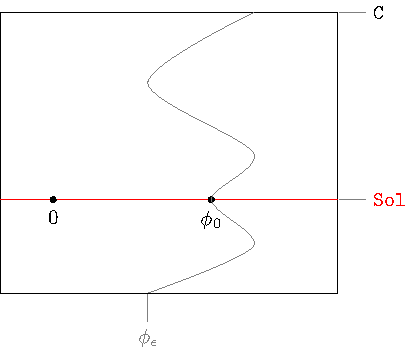
\includegraphics[width=\textwidth]{../Pictures/GeometricPicture0}
        \end{minipage}
        \begin{minipage}{0.5\textwidth}
            \begin{itemize}
                \item in this case the set $\Conf$, space of kinematic configurations, is a linear space and 
                    For the sake of simplicity we depict it as a plane, neglecting the complexities related to infinite-dimensional manifolds.
                \item Consequently, the space of solutions $ \Sol$ is a linear submanifold, in our picture a line, containing the section $0$.
                \item a variation is a parametrized curve on $\Conf$
            \end{itemize}
        \end{minipage}

\item 
        \begin{minipage}{0.4\textwidth}
            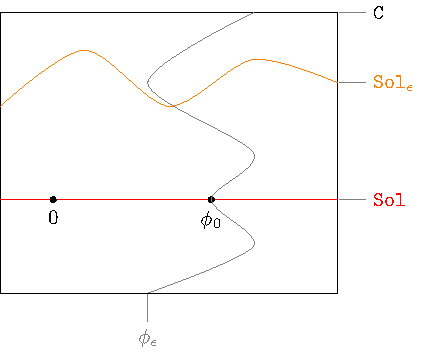
\includegraphics[width=\textwidth]{../Pictures/GeometricPicture1}
        \end{minipage}
        \begin{minipage}{0.5\textwidth}
            \begin{itemize}
                \item Peierls procedure prompt us to consider a disturbance (time compact supported lagrangian) both through its Eul-Lag operator than its lagrangian functional.
                \item     Since $Q_\chi$ is generally not linear,
                 we depict the space $\Sol_\epsilon$ of solutions of the disturbed dynamics equation $Q_{\Lagrangian + \epsilon \chi}$ as an arbitrary curve.\\
                    Without any loss of generality we  neglect the possibility that $\Sol \cap \Sol_\epsilon \neq \emptyset$ in this picture.
            \end{itemize}
        \end{minipage}
        
\item 
        \begin{minipage}{0.4\textwidth}
            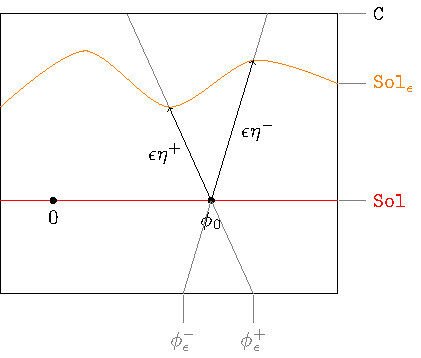
\includegraphics[width=\textwidth]{../Pictures/GeometricPicture2}
        \end{minipage}
        \begin{minipage}{0.5\textwidth}
            \begin{itemize}
                \item    Among all the possible linear variations of $\phi_0$, we consider the two variations $$\phi_\epsilon^\pm = \phi_0 + \epsilon \eta_\pm$$ matching the condition to lay on $\Sol_\epsilon$ at the first order in $\epsilon$.
                \item that is such that $\eta_\pm$ are the unique solution of Eq. \ref{PeierlJacobiEqLin}
                    $$ \eta_\pm = G^\pm \left( - Q_\chi \phi_0 \right) $$
                    determined by the fixed perturbation $\chi$.
                \item in layman terms this object quantifies how much the imperturbed solutions $\phi_0$ fails to be a solution of the disturbed equation of motion
            \end{itemize}
        \end{minipage}

\item The last ingredient is the effect operator acting on generic differentiable functionals on the systems.\\
        \begin{minipage}{0.4\textwidth}
            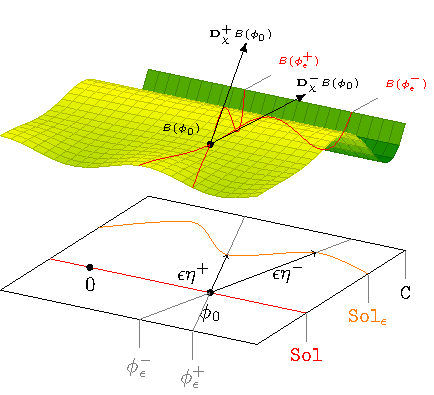
\includegraphics[width=\textwidth]{../Pictures/GeometricPicture3}
        \end{minipage}
        \begin{minipage}{0.5\textwidth}
            \begin{itemize}
                \item  Such functional can be depicted as an hypersurface on the plane $\Conf$
                \item ( according to this the solutions space can be regarded as extrema of the action $\mathcal{O}_\Lagrangian$)
                \item Effect operator  $\EffectOp_\chi^\pm B$ , effect of $\chi$ on $B$ evaluated in $\phi_0$, is formally a directional derivative in the direction of $\phi_\epsilon^\pm$ calculated in point $\phi_0$.
                \item that corresponds to the slope of this tangent vector.
            \end{itemize}
        \end{minipage}
        \item finally, considering a second disturbance and its corresponding lagrangian functional, we can conclude that the PB compute the difference between the slopes of the two function $$\mathcal{O}_\omega ( \phi_\epsilon^\pm)$$ which can be seen as a real function on the single variable $\epsilon$, calculated in $\epsilon=0$.
        \item Let me stress again that $ \phi_\epsilon^\pm$ are not arbitrary but they are two specific variations associated to $\chi$ and are the crucial part of the Peierls' procedure.
        \item Visually we can say that PB between $\chi$ and $\omega$ vanish in three cases:
        \begin{enumerate}
            \item The two curves $\mathcal{O}_\omega ( \phi_\epsilon^\pm)$ have the same derivative in $\phi_0$.
            \item The starting solution $\phi_0$ is also a solution of $Q_\omega$.\\
                (In this case, corresponds to $\phi_0$  an extremum of $\mathcal{O}_\omega$ thus its derivative vanishes according to each variations passing trough $\phi_0$)
            \item The starting solution $\phi_0$ is also a solution of $Q_\chi$.\\
                (In this case, the two perturbation $\phi_\epsilon^\pm$ are degenerate since they correspond to a transformation along a symmetry of the system )
        \end{enumerate}

    \end{itemize}
    \subsection{Considerations}
    \begin{itemize}
    \item In other words the PB compute how change the value of a Lagrangian functional when the dynamic configuration on which it's evalutated get shifted.\\
    The shift is  not arbitrary but it's determined by an infinitesimal change in the Lagrangian of the (unperturbed) system.
    \end{itemize}
    \newpage
    \section{Extension to Non-Linear Theories}
    \begin{itemize}
        \item in what shown is clear that green-hyperbolicity of motion operator $P$ plays a mayor role.
        \item however, the procedure can be stated even in presence of non-linear fields.\\
        that is when the motion operator and the configuration bundle are not necessarily linear.
        \item the crucial point of the procedure was to select, among all the possible solutions of perturbed motion $P_\epsilon$, those configurations which can be constructed by a variation of a given solution of the non-perturbed dynamics
        \item in this sense the problem of searching such variations in $\Conf$ results in a linearization\\
        \begin{minipage}{0.4\textwidth}
                   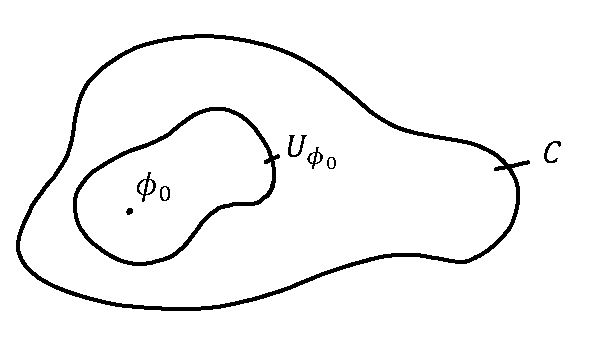
\includegraphics[width=\textwidth]{../Pictures/Linearization} 
        \end{minipage}
        \begin{minipage}{0.5\textwidth}
            \begin{itemize} 
                \item Finding the variation of solution $\gamma_0\in \Sol$ solving the disturbed motion equation
                \item is equaivalente to search the intersection between a local neighbourhood of $\gamma_0$ with $\ker(P_\epsilon)$
            \end{itemize}
        \end{minipage}    
        \item working patchwise, under a particular coordinate representationm we can define a local infinitesimal variation by acting on the components
        $$\gamma_\lambda ^{\, i}(x) = \gamma_0^{\, i}(x) + \lambda \eta^i(x) \qquad \forall x\in \pi(A) $$
        searching those local sections  which solve the perturbed equation up to the first order
        $$\big[ P_\epsilon \big] \gamma_\epsilon^{\,i} = o(\epsilon)$$
        \item we can tune the two modulation parameter $\lambda, \epsilon$ to be the same without lose of generalization
        \item passing through the linearization of operator P we obtain again a Jacobi Equation
        $$\biggr[P_{\gamma_0}^{\, lin} \biggr] \eta^i(x) = -\biggr(Q_\chi(\gamma_0)\biggr)(x)$$
        from this point the Peierls procedure could be carried on as before.
    \end{itemize}
    \newpage
    \section{Symplectic Structure derived by Peierls Brackets}
    \begin{itemize}
        \item How do we come from the PB to the claimed symplectic structure of the linear field system?
        \item let me first remark that the system under examination: is $$(E,\Lagrangian)$$ Linear lagrangian systems with $E$ vector bundle on globally hyperbolic spacetime.
        
        \item in order to complete the construction we have to ask for some technical requirements. 
    \end{itemize}
    \subsection{Pairing}
    \begin{itemize}
        \item a further technical requirement is the definition of an inner product on the configuration bundle.
        \item such that the induced pairing on the compactly supported sections
        \begin{itemize}
            \item         that is the bilinear function
            $$ (X,Y) = \int_M <X,Y>_x d\mu(x)$$
               where $d\mu = d\textrm{Vol}_\mu$ is the volume form induced by the metric and the orientation on $M$
            \item minimal domain in which this definition makes sense is
            $$ \dom\big( (\cdot, \cdot) \big) =
                       \big\{(X,Y) \in \Gamma^\infty(E) \times \Gamma^\infty(E) \; \big\vert \,  <X,Y>_x \in L^1(M,\mu)\big \} $$
        \end{itemize}
        \item (according to this pairing) the dynamics operator $P$  is formally self-adjoint
        $$(X,PY) = (PX,Y) \qquad \forall X,Y \in \Gamma_0$$
        \item the reason is that we will need the property of existence of uniqueness of the Green Operators $G^\pm$ and furthermore of the  causal propagator $E$ (\emph{Advanced minus Retarded operator}) the operator:
                $$
                    E \coloneqq G^-  - G^+ : \Gamma_{tc}(E) \rightarrow \Gamma(E)
                $$
    \end{itemize}
        

    
    \subsection{Space of Classical Observables}
    \begin{itemize}
        \item the first step to construct a symplectic space for our system is to identify the set that we want to endow with a symplectic form.
        \item this construction is achieved by the identification of the space of \emph{Classical Observables}
        \item A question could be raise spontanously:\\
        I said that i'm looking for a symplectic space then why am I starting form observables? \\
        (that are commonly related to the poisson structure?)
        \item The answer is that we are mimicking what happens in linear ordinary mechanical systems.
        \item in that case the symplectic structure is exactly reproduced from the phase space to the sub Poisson Algebra of the linear functional constructed from the(dual) correspondence
        $$ y \in \Phase \quad \mapsto \quad \omega(y,\cdot) \in \Obs_{\textrm{lin}} = \Phase^* $$
        \item from that should be clear the pivotal role of the Pairing
        \item (JUMPING STRAIGHT TO THE CONCLUSION)\\
        We can say that the suitable space to be endowed with a symplectic structure (The Classical phase space of the linear field)
        will be the set
        $$\frac{\Gamma_0}{P\Gamma_0} $$
        this is in a one-to-one correspondence with the space of (linear) classical observable on the space of dynamics configurations $\Sol$
        $$ \Obs = F\left( \frac{\Gamma_0}{P\Gamma_0}  \right) =\left\{ F_{[f]}(\phi) = F_f(\phi) \quad \forall \phi \in \Sol \; \forall f \in [f] \in \Gamma_0/P\Gamma_0 \right\} $$
    \end{itemize}
    \subsection{Construction of $\Obs$ is achieved in three steps}
    \begin{enumerate}
        \item 
            \begin{itemize}
                \item we start defining the class of off shell functional $\emph{Pre-observable}$:
                    $$\Obs_0 \coloneqq \left\{ F_f:\Conf \rightarrow \Real \quad \left\vert \quad f \in \Gamma_0 \; ; \; F_f(\phi) = (f,\phi) \quad\forall \phi \right. \right\}$$
                \item can be proved (surjectivity by definition and injectivity ad absurdum) that the map
                $$F: \Gamma_0 \rightarrow \Obs_0 \qquad f \mapsto F_f$$
                is bijective
                \item more interesting is the fact that $\Obs_0$ statisfy the separability condition
                $$ \forall \phi, \psi \in \Conf \quad \exists f \in \Gamma_0 \quad \textrm{s.t.} \quad F_f(\phi) \neq F_f(\psi)$$
                usually required for a well-defined set of observables.
            \end{itemize}
        \item
            \begin{itemize}
                \item on the other hand, if we consider the restriction of such functionals from $\Conf$ to $\Sol$,
                the mapping 
                $$ F^\Sol : \Gamma_0  \ni f \mapsto (f,\cdot) \big\vert_\Sol $$
                fails to be faithful.
                \item Precisely,  it is no more injective
                $$ \ker(F^\Sol) = P \left( \Gamma_0^\infty \right)$$
                \item left $\supseteq$ right because:
                $$ F_{P\tau} ( \sigma ) = ( P\tau, \sigma ) = (\tau , P\sigma) = 0 \qquad \forall \sigma \in \Sol , \; \forall \tau \in \Gamma_0$$
                \item left $\subseteq$ right because: \\
                (exploiting $\exists ! E$ and skew-self-adjointness of $E$
                $$ \forall \tau \in \ker(F^\Sol) , \; \forall \sigma \in \Sol \quad \Rightarrow \quad 0 = ( \tau , E \sigma) = (-E\tau, \sigma)$$
                the non degeneracy of the pairing implies
                $$ E\tau = 0$$
                but
                $$ \ker(E\vert_{\Gamma_0}) = P\Gamma_0 $$
                since
                $$ PE f = 0 \quad \forall f \in \Gamma_\textrm{tc} $$
            \end{itemize}
        \item
            \begin{itemize}
                \item due to the degeneracy of this map $F^\Sol(\Gamma_0)$ could not be a good set of observable.
                \item the simplest way to overcome this problem is to identify all those elements determining the same observable functional on $\Sol$.
                \item that is considering the quotient space $$\frac{\Gamma_0}{P \Gamma_0}$$
                and transporting the mapping $F$ yelding the functional of thi space.
                \item that is defining
                $$F: \frac{\Gamma_0}{P \Gamma_0} \rightarrow \Obs \qquad 
                \textrm{s.t.} \qquad
                [f] \mapsto F_{[f]}(\phi) = F_f(\phi) \quad 
                \forall \phi \in \Sol , \; \forall f \in [f] \in \Gamma_0 / P \Gamma_0 $$
                \item by definition this functional is well-defined (that is independent from the choice of the representative) on $\Sol$
                \item mapping is bijectivite
                \item the separability condition is mantained a fortiori of separability of $\Obs_0$
            \end{itemize}
        \item (Conclusions)
            \begin{itemize}
                \item Thus we can identify the space of classical observables with that quotient space
                $$ \Obs \simeq \frac{\Gamma_0^\infty}{P \gamma_0^\infty} $$
                \item through the UNIQUE operator $E$ can be proved a further one-to-one correspondence between this quotient space $\Gamma_0 / P \Gamma_0$ and the space of dynamics configurations $\Sol$.\\
                Namely:
                \begin{itemize}
                    \item propagator determine a  well-defined on the equivalence classes as  
                    $$ E[f] =  E f $$
                    because
                    $$ E(f + P h ) = E f  \quad \forall f,h \in \Gamma_0 \subset \dom(E)$$
                    \item $ P E f = 0 $ by definition of Green operators.
                \end{itemize}
                \item keeping in mind the correspondence between solution  - initial data  - phase space in ordinary classical mechanics,
                this quotient space is a great candidate  to be the phase space of the system
            \end{itemize}
    \end{enumerate}
    \subsection{Symplectic form on $\Obs$}
    \begin{itemize}
        \item Ok, we have pointed out the set.\\
        Now we have to equip it with a suitable symplectic structure.\\
        Here come handy the Peierls procedure
        \item Recalling that
        \begin{itemize}
            \item The Lagrangian functionals on $\Conf$ was defined through a distribution in order to keep under control the behaviour on configurations with unlimited support.
            \item restricting ourselves to the compact-supported configurations (from $\Sol$ to $\Gamma_0$) we can consider the symplified form of the functional:
            $$ \mathcal{O}_\Lagrangian ( \phi_0) ) \int_M \Lagrangian(\phi_0) d \mu \qquad \forall \phi \in \Gamma_0$$
            \item the effect could now be defined as the limit of the incremental ratio (it is no more necessary to consider derivative in distributional sense) and the Peirels takes the same form as before:
            $$\{\chi, \omega \}(\phi_0) \coloneqq \EffectOp_\chi^- \mathcal{O}_\omega (\phi_0) - \EffectOp_\chi^+ \mathcal{O}_\omega(\phi_0) $$
        \end{itemize}
        \item the key idea , in order to transport this construction to the space $\Obs$, is that any compactely supported section $\phi \in \Gamma_0$ can be made to correspond a particular class of Lagrangian densities
        $$ \phi \in \Gamma_0^\infty \quad \mapsto \Lagrangian_\phi \big[\cdot \big] ( x ) = <\phi, \cdot>_x $$
        exploiting again the bundle inner product
        \item thus, the associated lagrangian functional on $\Gamma_0$ is simply
        $$                             \mathcal{O}_{\Lagrangian_\phi} (\cdot ) = \int_M  <\phi, \cdot>_x d\mu(x) = (\phi, \cdot) = F_\phi (\cdot)$$
        \item and the corresponding Eul-Lag operator results
        $$Q_{\Lagrangian_\phi}= \biggr( \nabla_\mu \big( \frac{\partial \Lagrangian}{\partial ( \partial_\mu \phi)} \big) - \frac{\partial \Lagrangian}{\partial \varphi} \biggr) = - \frac{\partial \Lagrangian_\varphi}{\partial \varphi} = -\frac{\partial}{\partial \varphi} (\phi, \varphi) = -\phi$$
        (the operator mapping the whole space $\Conf$ to  "minus $\phi$")
        \item the effect operator computed on a pair of this very particular Lagrangians results ( $\forall     \phi_0\in \Sol$):
        \begin{align}
            \EffectOp_{\Lagrangian_\alpha}^\pm \big( \mathcal{O}_{\Lagrangian_\beta} \big)& (\phi_0) 
            \stackrel{(a)}{=}
             \lim_{\epsilon \rightarrow 0} \biggr( \frac{1}{\epsilon}\big(F_\beta ( \phi_{\epsilon \Lagrangian_\alpha}^\pm) - F_\beta(\phi_0) \big) \biggr) 
            \stackrel{(b)}{=}
            \lim_{\epsilon \rightarrow 0} F_\beta\left( \frac{ \phi_{\epsilon \Lagrangian_\alpha}^\pm- \phi_0}{\epsilon} \right)  
                        \nonumber\\
            &\stackrel{(c)}{=} (\beta, \eta_\pm) 
                \stackrel{(d)}{=} \big( \beta, - G^\pm (Q_{\Lagrangian_\alpha} \phi_0 ) \big) 
                \stackrel{(e)}{=} ( \beta, G^\pm \alpha) \nonumber
        \end{align}
        \begin{footnotesize}\begin{itemize}
            \item    (a) Lagrangian functional coincide with $F_\alpha$
            \item (b) explotiing linearity and continuity of F
            \item (c) exploting difinition of disturbed solutions and $F$
            \item (d) exploiting the unieques of $\eta$ which follows from the green-hyperbolicity
            \item (e) using explicit expression of $Q_{\Lagrangian_\alpha}$
        \end{itemize}\end{footnotesize}
        \item Notice that the dependency from test solution $\phi_0 \in \Sol$ has disappeared!
        \item Thus, considering only lagrangian constructed from compact supported sections, the peierls brackets have induced a bilinear map on $\Gamma_0$
        $$                             \tau\left( [f] , [h]\right) = \{\Lagrangian_f , \Lagrangian_h\} = \big( f , (\GreenAdv - \GreenRet)h \big) = \big(f, E h\big) \qquad \forall f,h \: \Gamma_0^\infty (E)$$
        \item notice that at this point the condition of lagrangian system is become completely ancillary.\\
        In fact it's customary in the modern literature (see DeWitt for example) to overlook at the origin of this object jumping directly to this expression as a postulate.
        \item we have almost done.
        The last effort is to transport this bracket to the set $\Phase = \Gamma_0 / P \Gamma_0$ defined above.
        \item the problem is that the brackets $\tau$ (PB restricted to $\Gamma_0$) are degenerate on $\Obs_0$ since:
        $$ \forall f = P h \qquad (f, E g ) = ( P h , E g ) = ( -E P h , g ) = ( 0 , g ) = 0$$
        \item This is actually an advantage since it allows to define such bilinear operator on the equivalence classes of $\Phase$ as
        $$ \tau \left( [\phi] , [\psi] \right) \coloneqq \tau \left( \phi , \psi \right)$$
        losing any dependency from the representative of the equivalence class.
        \item Properties of $\tau$:
        \begin{itemize}
            \item is bilinear from bilinearity of pairing and linearity of $E$
            \item is not degenerate
                $$(f , Eh) = 0 \quad \forall f \in \Obs_0 \qquad \stackrel{(a)}{\Leftrightarrow} \qquad 
                E h = 0 \qquad \stackrel{(b)}{\Leftrightarrow}  \qquad 
                \exists f \;\textrm{s.t.}\; h = P f$$
                \begin{footnotesize}\begin{itemize}
                    \item    (a) non degeneracy of the pairing
                    \item (b) $[h] = [Pf] = [0]$
                \end{itemize}\end{footnotesize}            
            \item skew-symmetric from the symmetry of the pairing
                $$ \tau(f,h) = ( f , E h) = - (E f , h ) =  - (h , E f ) = -\tau(h , f ) $$
        \end{itemize}
    \end{itemize}
    \newpage
    \section{Conclusions}
    \begin{itemize}
        \item as Claimed the pair $$(\Obs, \tau)$$ is a proper symplectic space associated to the linear field system with a symplectic form induced by the Peierls procedure.
        \item from this point the algebraic quantization scheme can be easily applied (construction of algebra of observables and Hadamard state)
        \item    Within my thesis I've tried to keep my mathematical formalization to an intermediate degree of sophistication.\\
        Currently are under examining further extensions of the Peierls construction to non-Lagrangian fields or to systems with Gauge freedom, all of these are based on the variational bi-complex formalism. \\
    We have preferred to keep my discussion to this level since the current lack of bibliography on the theme is hindering the recognition of the role of the Peierls often relegating it to a mere "mathematical trick".
        \item Its main drawback is a lack of mathematical rigor when we have used formal extrapolation of techniques from ordinary calculus on manifolds to the infinite-dimensional setting
        \item transforming such formal results into mathematical theorems is a separate problem\\
        applications to this topic of modern results in non-linear global analysis are currently not extensively investigated.
    \end{itemize}

    \end{document} %\/\/\/\/\/\/\/\/\/\/\/\/\/\/\/\/\/\/\/\/\/\/\/\/\/\/\/\/\/\/\/\/\/\/\/\/\/\/\/\/\/\/\/\/\/\/\/\/\/\/\/\/\/\/\/\/\/\/\/\
    %\/\/\/\/\/\/\/\/\/\/\/\/\/\/\/\/\/\/\/\/\/\/\/\/\/\/\/\/\/\/\/\/\/\/\/\/\/\/\/\/\/\/\/\/\/\/\/\/\/\/\/\/\/\/\/\/\/\/\/\/\/\/\/\/\/\/\/\/\/